JWT steht für "JSON Web Token" und repräsentiert einen offenen Standard (RFC 7519). Er ist zur Authentifizierung und Autorisierung gedacht, dieser Token kann sowohl vom Server als auch vom Client ausgelesen werden. Er kann verwendet werden um Daten sicher zwischen verschiedenen Anwendungen zu übermitteln. Durch die Signatur des JWT kann immer sichergestellt werden, dass nichts vom Inhalt manipuliert wurde.


\subsection{Wie ist ein JWT aufgebaut?}
Ein JWT ist grundlegend in drei Bereiche gegliedert:

\begin{itemize}
\item \textbf{Header}
\item \textbf{Payload}
\item \textbf{Signatur}
\end{itemize}

Es ist grundsätzlich ein einfacher Zeichenstring welcher in drei verschiedene Teile gegliedert wird, welche jeweils nur mit einem Punkt getrennt sind und mit Base64 kodiert sind. Ein Token lässt sich in folgender Form darstellen:

\begin{lstlisting}
Header.Payload.Signatur
\end{lstlisting}


\begin{figure}[h!]
    \centering
    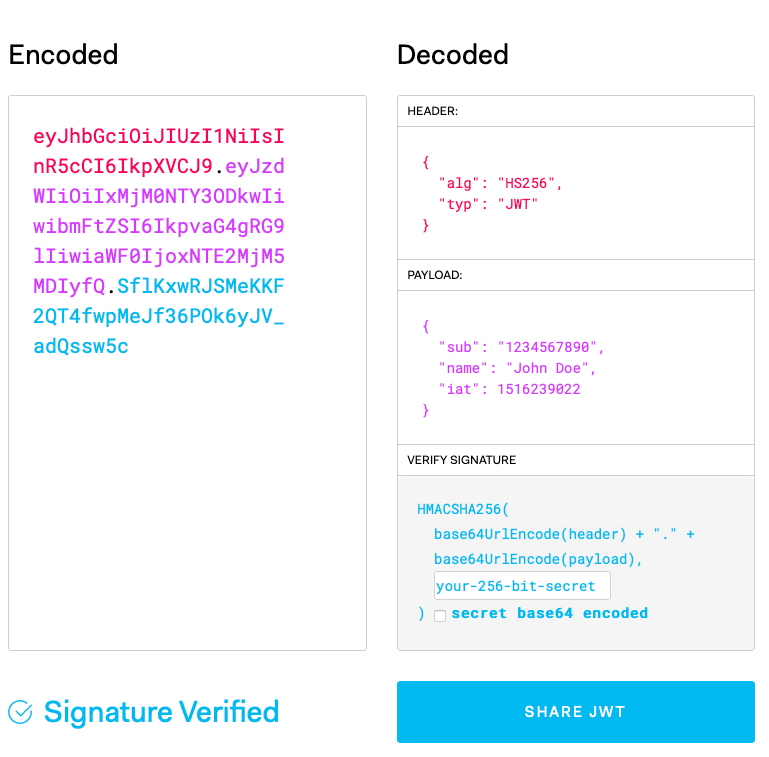
\includegraphics[width=0.6\textwidth]{pics/jwt.png}
    \caption{JSON Web Token}
    \label{fig:enter-label}
\end{figure}

\subsubsection{Wie wird ein JSON Web Token implementiert?}

Als erstes muss das dafür notwendige Package mit folgendem Befehl installiert werden:

\begin{lstlisting}
npm install jsonwebtoken
\end{lstlisting}


\begin{lstlisting}
const jwt = require('jsonwebtoken')

const generateToken = (email) => {
  return jwt.sign(
    { email },
    'secretkeyappearshere',
    { expiresIn: '100h' }
  )
}

const verifyToken = (token) => {
  let payload
  try {
    payload = jwt.verify(token, 'secretkeyappearshere')
  } catch (e) {
    next()
  }
  return payload
}
\end{lstlisting}

Zuerst wird der JSON Web Token mit Hilfe der Funktion "generateToken" generiert. Hierfür wird die E-Mail Adresse als Parameter übergeben und als Payload mitgegeben. Außerdem wird noch ein Expire Date gesetzt auf in diesem Fall 100 Stunden.

In der Funktion "verifyToken" können JSON Web Tokens validiert werden. Mit

\begin{lstlisting}
    payload = jwt.verify(token, 'secretkeyappearshere')
\end{lstlisting}

wird der Token validiert und geschaut ob dieser noch gültig ist wird hier ein Fehler returned wird einfach in die nächste API Middleware weitergegangen. Ist dieser Vorgang erfolgreich wird die Payload, also in diesem Fall die E-Mail Adresse zurückgeschickt.


\subsubsection{Header}

Der Header wird auch als JOSE (JSON Object Signing and Encryption) bezeichnet. In diesem sind ausschließlich Informationen über die Signierung und Verschlüsselung des JWT enthalten.


Typischerweise enthält die Struktur eines JWT-Headers eine Information über den Algorithmus, welcher zur Erstellung der Signatur verwendet wurde, sowie eine Definition, dass es sich um ein Json Web Token handelt. Dabei ist zu beachten, dass die Angabe des Typs optional ist, jedoch häufig auf "JWT" festgelegt wird. Dies ist besonders relevant für Anwendungen, die auch andere Typen, wie beispielsweise einen Access Token, akzeptieren, welcher jedoch in einer ähnlichen Datenstruktur vorliegt, um die verschiedenen Typen leicht voneinander unterscheiden zu können.

\begin{lstlisting}
{
  "alg": "HS256",
  "typ": "JWT"
}
\end{lstlisting}

\subsubsection{Payload}
Der zweite Part des JSON Web Token ist die Payload. Diese beinhaltet drei verschiedene Arten von Claims. 
Registrierte, Public und Private Claims

In den registrierten Claims sind zum Beispiel Sachen wie der Aussteller (iss) und die Ablaufzeit (exp) festgelegt.

Die Public Claims können nach Belieben definiert werden. Um jedoch Kollisionen zu vermeiden sollte der Name nicht gleich sein wie bei den registrierten Claims.

Die Privaten Claims sind individuelle Ansprüche, die erstellt wurden, um Informationen zwischen Parteien auszutauschen, die sich darauf einigen, sie zu verwenden, und die weder registrierte noch öffentliche Ansprüche sind.


\subsubsection{Signatur}

Der dritte Teil des JWT ist die Signatur diese ist in RFC 7515 definiert. Es kann sein das kein Algorithmus definiert wurde in diesem Fall entfällt die Signatur. Es gibt allerdings ganz seltene Fälle in denen dieses Verhalten erwünscht ist. 



Das zweite Verfahren wurde bereits erläutert. Dabei wird ein Algorithmus wie HS256 oder RS256 verwendet, um anhand der Daten einen eindeutigen Wert zu generieren und mögliche Manipulationen der Payload auszuschließen.



Das dritte Verfahren geht einen zusätzlichen Schritt weiter, indem es auf Verschlüsselung (JWE) setzt. Hier wird die Payload erneut mit einem privaten Schlüssel verschlüsselt und muss entsprechend entschlüsselt werden, um wieder im Klartext lesbar zu sein.

\subsection{Was ist ein Session Cookie?}


Ein Sitzungscookie ist eine Variante von Cookies, die nach dem Schließen des Browsers direkt gelöscht wird und keine Informationen hinterlassen werden. Normalerweise enthält ein solches Sitzungscookie keine Informationen zur Identifizierung des Benutzers, sondern nur eine Sitzungs-ID.
Wenn in zwei Tabs also der gleiche Online Shop besucht wird, erkennt der Session Cookie, dass es sich gerade um die gleiche Sitzung handelt und stellt in beiden Tabs den selben Warenkorb zu Verfügung.

\subsubsection{Wie wird ein Session Cookie implementiert?}

\begin{lstlisting}
var cookieSession = require('cookie-session')
var express = require('express')

var app = express()

app.use(cookieSession({
  name: 'session',
  keys: [/* secret keys */],

  // Cookie Options
  maxAge: 24 * 60 * 60 * 1000 // 24 hours
}))
\end{lstlisting}

\subsubsection{Session Cookie vs JSON Web Token}

Der wohl größte Unterschied zwischen den beiden Autorisierungsmethoden ist, dass beim Session Cookie vom Server eine Session-ID generiert wird. Beim JSON Web Token hingegen, wird ein Access Token generiert.
Json Web Tokens ermöglichen eine sehr schnelle Autorisierung. Jedoch werden mehr Entwicklerinvestionen benötigt als beim Session Cookie. Auf der anderen Seite bieten Sitzungen stärkere Garantien dafür, dass jede einzelne Anfrage autorisiert ist, und sind einfacher sicher umzusetzen, aber ihr Engpass bei der serverseitigen Datenbankvalidierung geht mit einem Latenzoverhead einher, der das Benutzererlebnis für sehr reaktionsschnelle Anwendungen beeinträchtigen könnte.

\begin{lstlisting}
app.get("/", (req, res) => {
   console.log(req.session.id)      // get sessionId
   console.log(req.session.cookie)  // get cookie
})
\end{lstlisting}




https://medium.com/@prashantramnyc/difference-between-session-cookies-vs-jwt-json-web-tokens-for-session-management-4be67d2f066e

\cite{JWT_1}

\cite{JWT_2"}

\cite{JWT_3}
